\documentclass{article}
\usepackage[utf8]{inputenc}
\usepackage{geometry, parskip, hyperref, enumitem}
\usepackage{amsfonts, amsmath}
\usepackage{pgfplots, graphicx}
\usepackage{caption, subcaption}


\title{
    \textbf{ECE250: Signals \& Systems} \\
    \large{Assignment 2: Report}
}

\author{\href{mailto:divyajeet21529@iiitd.ac.in}{Divyajeet Singh (2021529)}}

\date{September 30, 2022}

\geometry{a4paper, left=25mm, right=25mm, top=25mm, bottom=25mm}
\pgfplotsset{compat=1.18}

\begin{document}
    \maketitle

    \textbf{Assumptions:}

    \begin{enumerate}
        \item The signal $u(t)$ is the unit-step signal, defined below: \begin{equation}
            u(t) = \begin{cases}
                1 & \text{ if } t \geq 0 \\
                0 & \text{ if } t < 0
            \end{cases}
        \end{equation}

        \item Since we cannot deal with \textit{continuous}-time signals in Python, I
        have assumed a very small time interval $dt = 0.01$ to plot the signals and
        perform the convolution.
    \end{enumerate}
    \vspace{5mm}

    \textbf{Notes:}

    \begin{enumerate}
        \item
        \textbf{Question: 1} asks us to plot the signals $x(t),\ h(t)$, and $y(t)$ for
        $t \in [0, 20]$. However, I have plotted the signals $x(t),\ h(t),$ and $h(-t)$
        for $t \in [-20, 20]$ for visualization as well.
    \end{enumerate}
    \vspace{1cm}

    \textbf{Question: 1}

    \begin{enumerate}[label=(\alph*)]
        \item Given the following signals $x(t)$ and $h(t)$:
        \begin{align}
            x(t) &= \cos{(t)} u(t) \\
            h(t) &= \frac{1}{4} \left( e^{-2t} - e^{-t} \right) u(t)
        \end{align}

        \begin{figure}[ht]
            \centering
            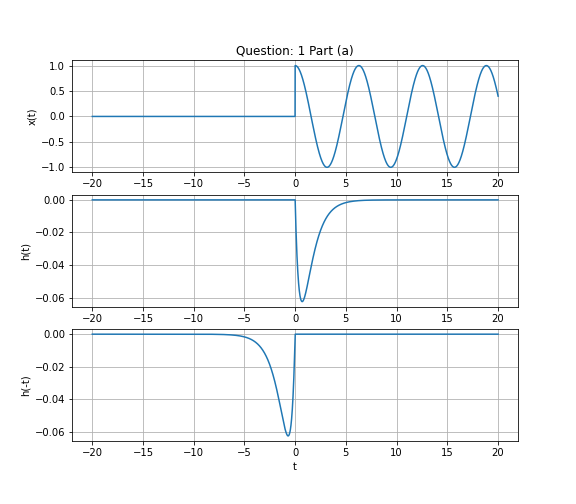
\includegraphics[scale=0.39]{./Assets/1-a-i.png}
            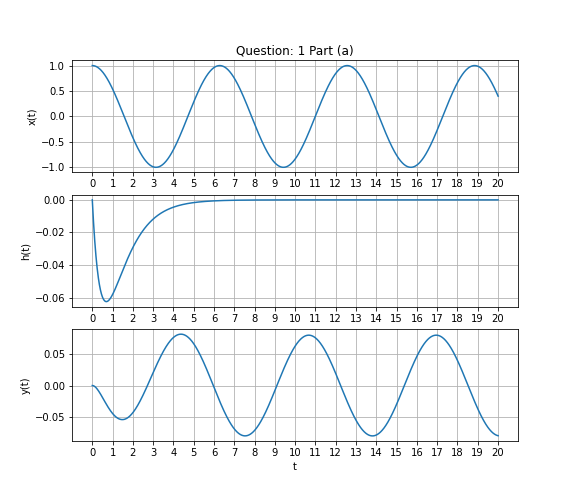
\includegraphics[scale=0.39]{./Assets/1-a-ii.png}
            \caption*{Subplots for \textbf{Question: 1 (a)}}
        \end{figure}
        \pagebreak

        \item
        Given the following signals $x(t)$ and $h(t)$:
        \begin{align}
            x(t) &= e^{-t} \sin{(t)} u(t)  \\
            h(t) &= \frac{1}{2} \left( e^{-t} - e^{-4t} \right) u(t)
        \end{align}

        \begin{figure}[ht]
            \centering
            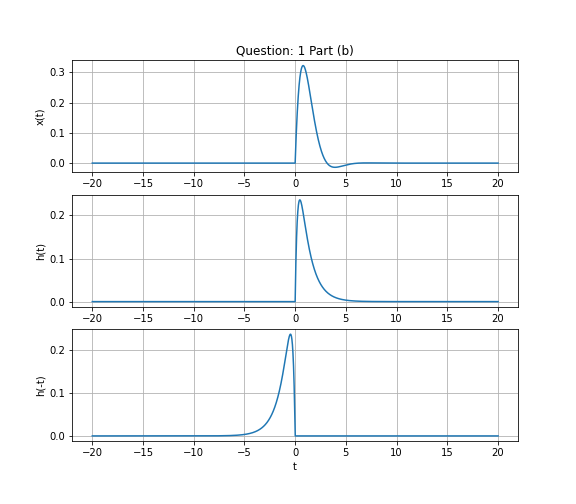
\includegraphics[scale=0.39]{./Assets/1-b-i.png}
            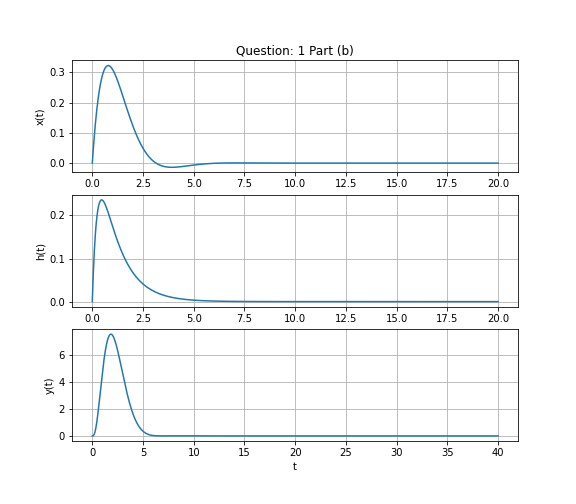
\includegraphics[scale=0.39]{./Assets/1-b-ii.png}
            \caption*{Subplots for \textbf{Question: 1 (b)}}
        \end{figure}
    \end{enumerate}

\end{document}